% %!TEX root = main.tex

\section{Introduction}

% \begin{figure}
% \centering
% \includegraphics[width=\linewidth]{figures/teaser/teaser.pdf}
% \caption{We propose a new method that estimates the camera field of view and the horizon line from a single image. We evaluate our proposed method alongside state-of-the-art techniques for single image geometric camera calibration. We performed a large-scale user study to understand the impact of calibration error on human perception, we using a human sensitivity measure obtained by our study.}
% \label{fig:teaser}
% \end{figure}

The first step for many vision and graphics tasks---ranging from 3D scene reconstruction to image metrology to photographic editing---is to geometrically calibrate the camera that captured the image~\cite{Hartley2004}. In this work, we are specifically interested in calibrating a camera from a single image of a natural scene, thereby precluding the use of multiple views of the scene or calibration targets. There is a extensive body of work even in this challenging setting; however, most approaches rely on detecting specific image features like vanishing lines~\cite{Lee2014}, coplanar circles~\cite{Chen2004} and repeated texture patterns~\cite{Schaffalitzky2000,Criminisi00,Pritts2014}, making them inapplicable to images without these features.

Inspired by the success of deep learning for related scene reconstruction tasks~\cite{choy20163d,bianco2017single}, we propose training a deep convolutional network to directly estimate camera parameters---more specifically the focal length, pitch and roll--from a single image. This is similar to recent work on CNN-based focal length~\cite{Workman2015a} and horizon estimation~\cite{Workman2016}. We significantly improve on their results by jointly estimating all the parameters and by training on sample images automatically extracted from a large-scale panorama dataset~\cite{Xiao2012}. We also analyze the features learned by the network to understand how it differs from pre-defined feature-based calibration.

While our calibration network produces state-of-the-art results, there are a number of cases where it fails. For images with no clear geometric or semantic cues, there is ambiguous evidence for what the ``right'' camera calibration parameters should be. In many situations, recovering the exact camera calibration may not even be required; for example, humans are known to tolerate strong deviations from realism in painting~\cite{Cavanagh2005} and digital composites~\cite{Farid2010}. This lead us to ask the question: \emph{how do humans perceive inaccuracies in geometric camera calibration}? To answer this, we conducted a large-scale user study to test the human perception of errors in camera calibration. We composited virtual objects into images using both ground truth calibration parameters as well as randomly perturbed parameters, and asked users to evaluate which image in each pair looked ``real'' to them. The results of this user study are described in sec.~\ref{sec:human_sensitivity_analysis}. To our knowledge, this is the first large-scale user study to systematically evaluate human perception of camera perspective. We use this data to design a new perceptual measure for calibration errors that we believe can prove to be important as we evaluate how precise our algorithms need to be for applications like augmented reality and 3D object composition.

While our calibration network was trained to minimize an entropy-based loss, we show that it also outperforms previous methods on our perceptual measure. In addition, we also demonstrate the use of our network for a wide range of applications, including 3D object insertion, calibration-based image retrieval and compositing.  

\newcommand{\exampleresultswidth}{0.195}
\begin{figure*}
\centering
\bgroup
% \def\arraystretch{0}
\setlength{\tabcolsep}{1pt}
\begin{tabular}{cccc|c}
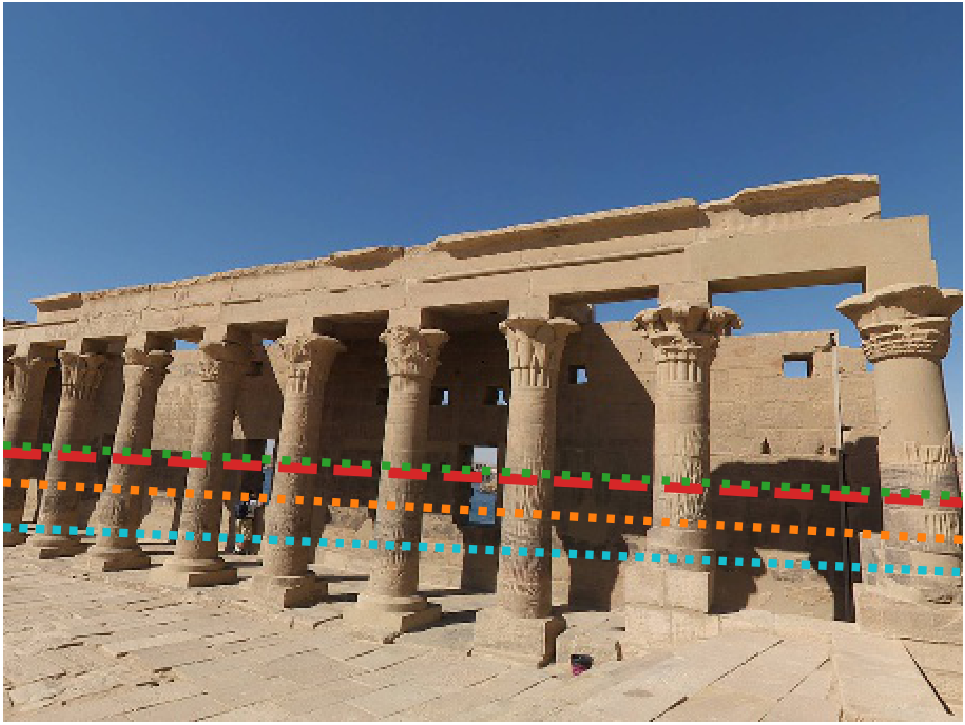
\includegraphics[width=\exampleresultswidth\linewidth]{figures/method/results/pano_addbhhhqoevobx_jpg-1.png} &
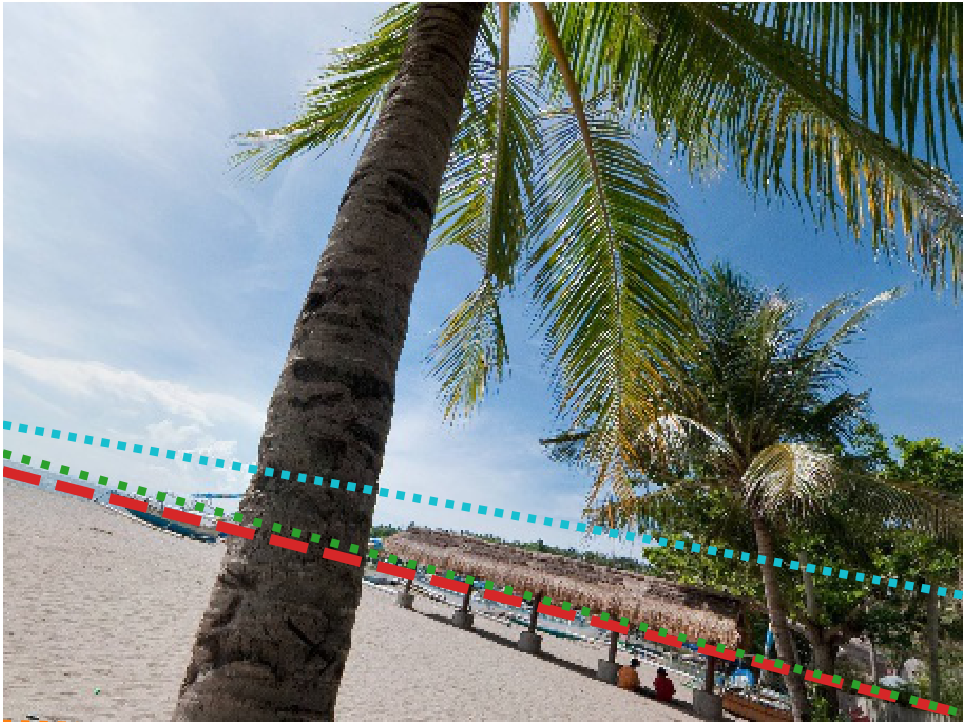
\includegraphics[width=\exampleresultswidth\linewidth]{figures/method/results/pano_addtdiecjavkue_jpg-3.png} &
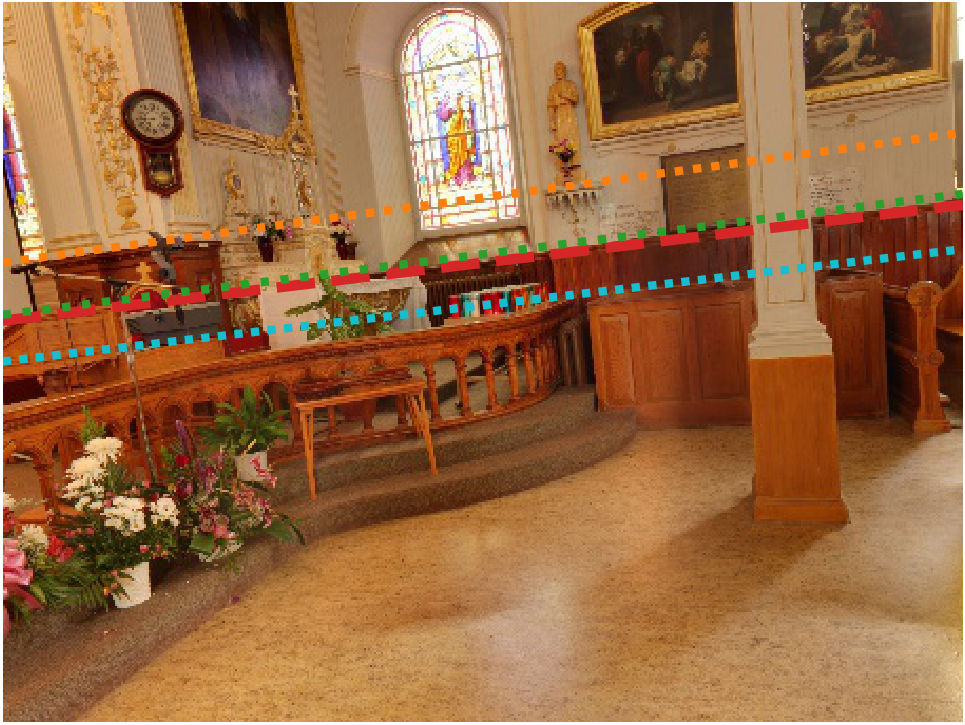
\includegraphics[width=\exampleresultswidth\linewidth]{figures/method/results/pano_adddhslzzqcooj_jpg-4.png} &
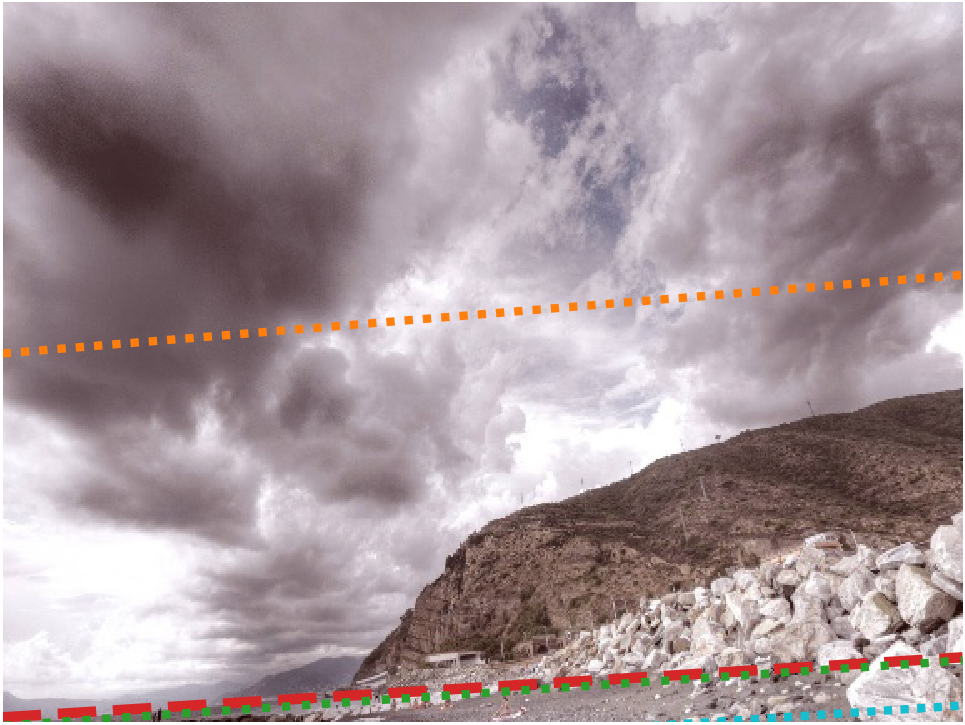
\includegraphics[width=\exampleresultswidth\linewidth]{figures/method/results/pano_addtfngrqwwyvb_jpg-6.png} &
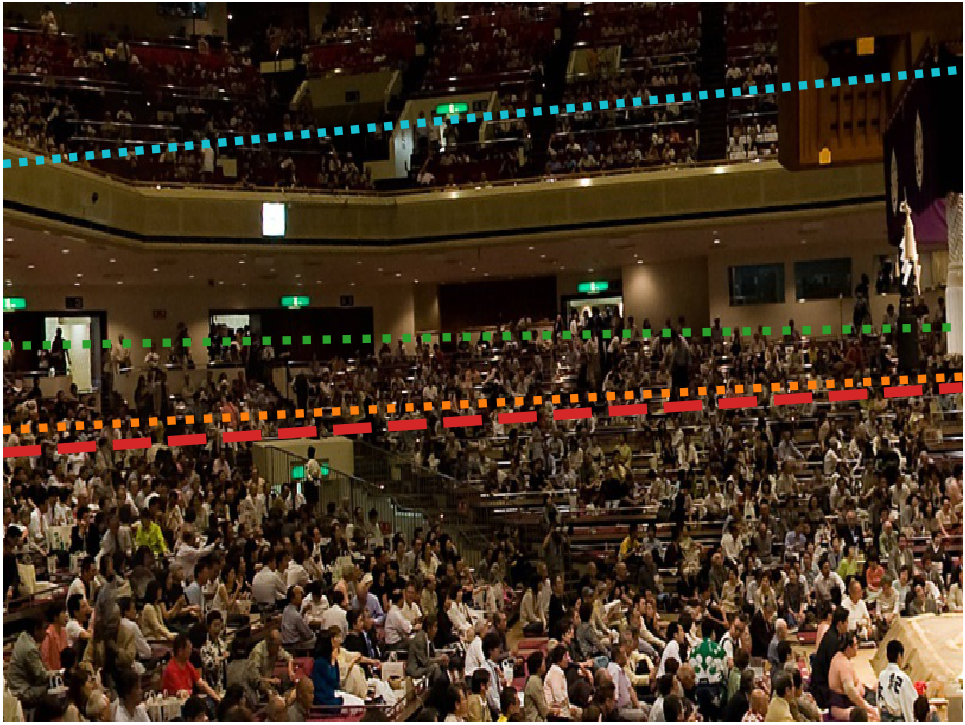
\includegraphics[width=\exampleresultswidth\linewidth]{figures/method/failures/pano_ayfpxwwfwgfweh_jpg-2.png} \\
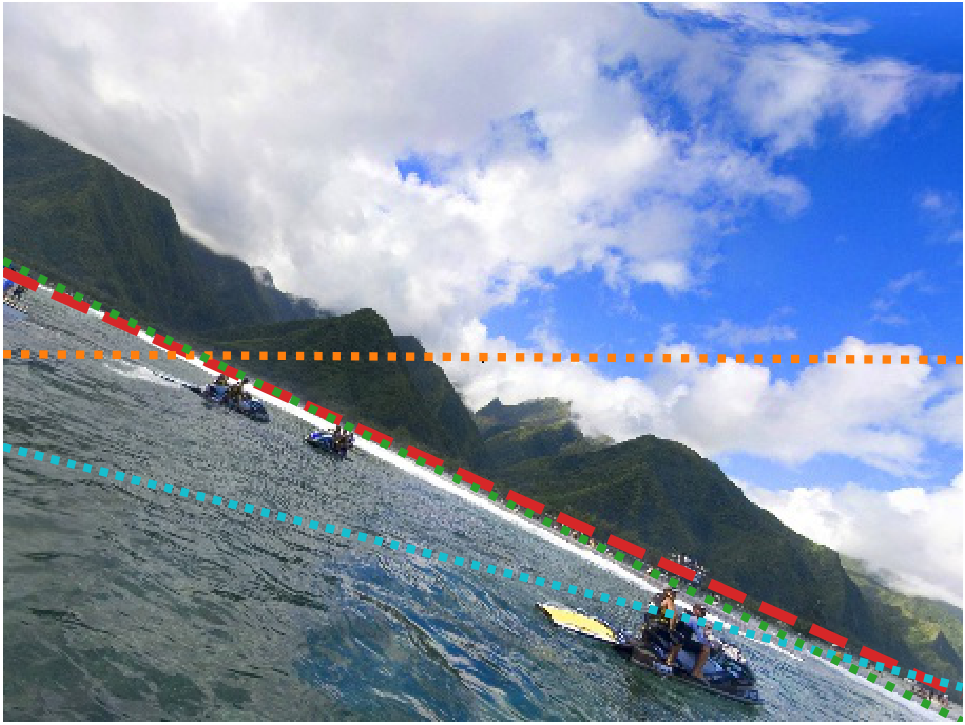
\includegraphics[width=\exampleresultswidth\linewidth]{figures/method/results/pano_addgasjevqjafh_jpg-1.png} &
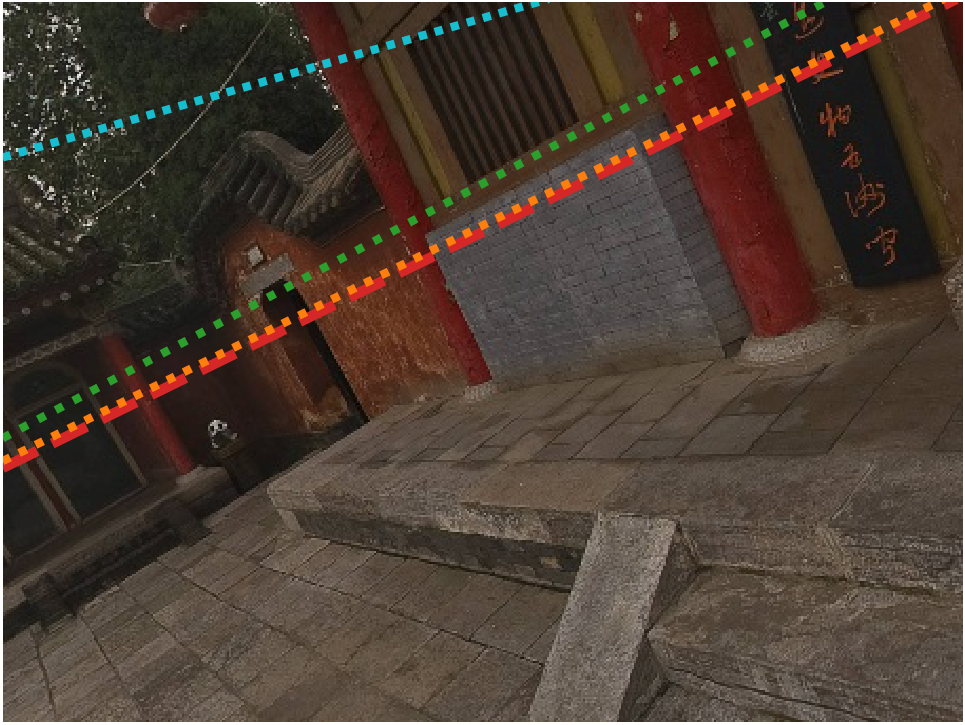
\includegraphics[width=\exampleresultswidth\linewidth]{figures/method/results/pano_addgtzfdddfgrh_jpg-2.png} &
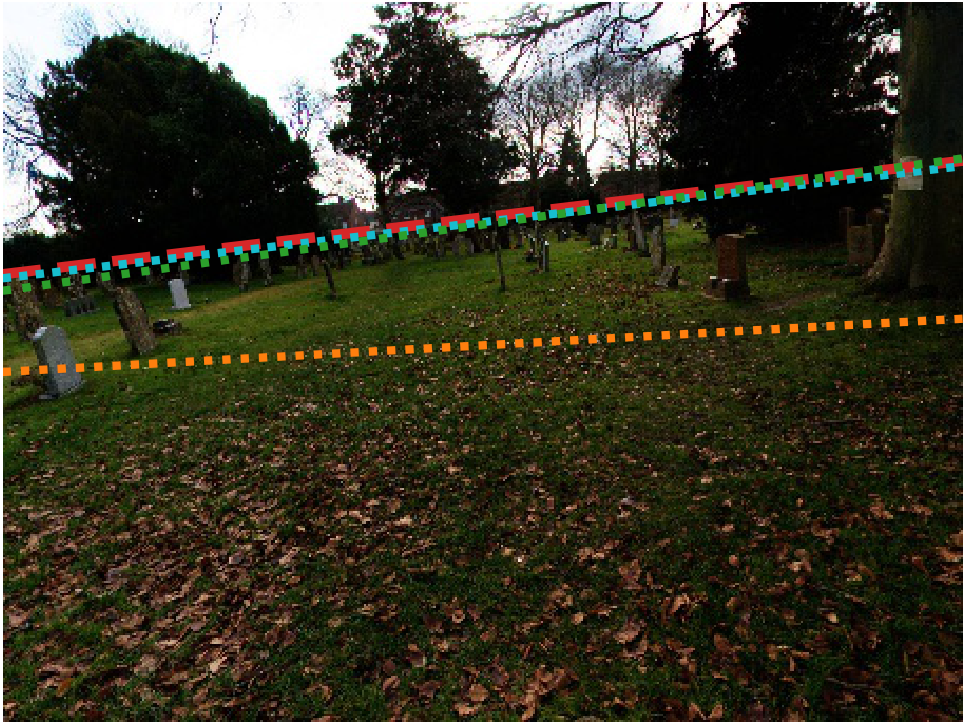
\includegraphics[width=\exampleresultswidth\linewidth]{figures/method/results/pano_addhxkomphqrlr_jpg-4.png} &
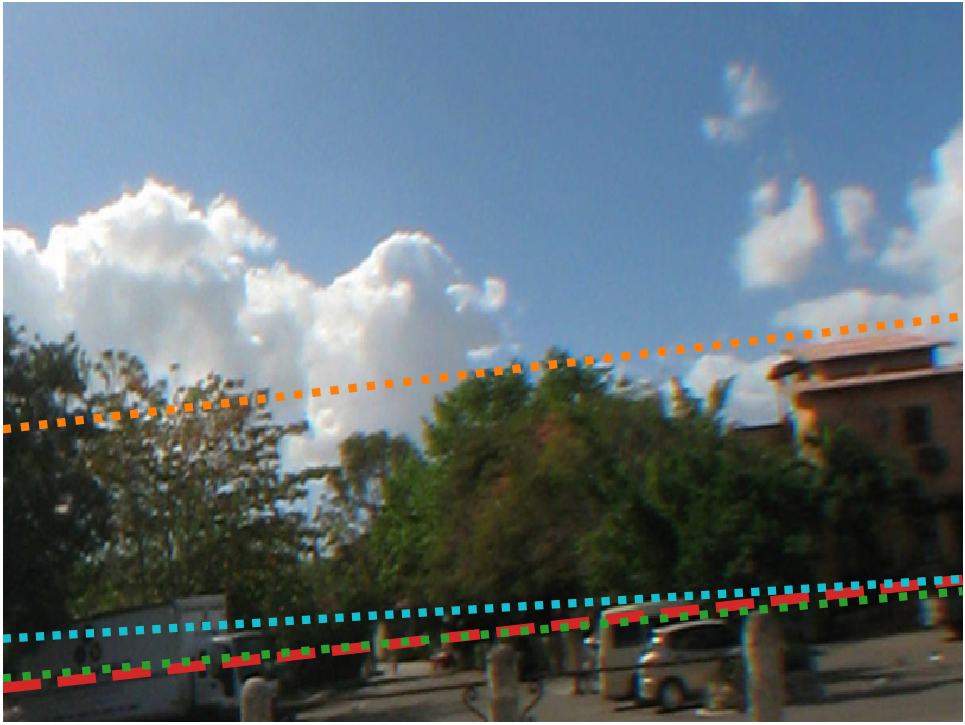
\includegraphics[width=\exampleresultswidth\linewidth]{figures/method/results/pano_ayfzatxlublfjc_jpg-5.png} &
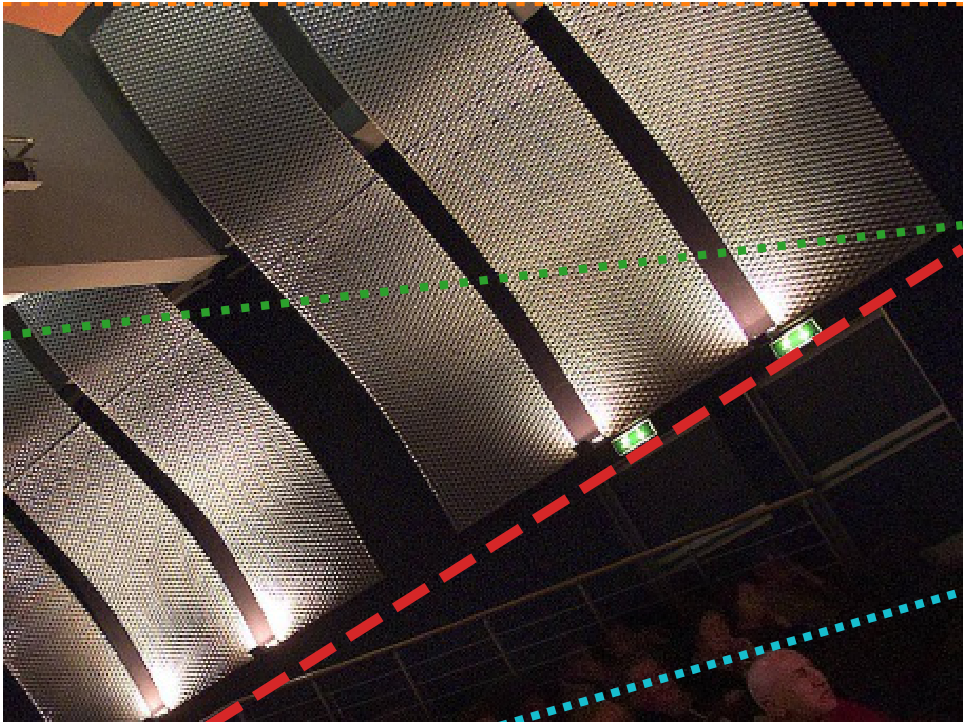
\includegraphics[width=\exampleresultswidth\linewidth]{figures/method/failures/pano_addwoduaropmic_jpg-4.png} \\
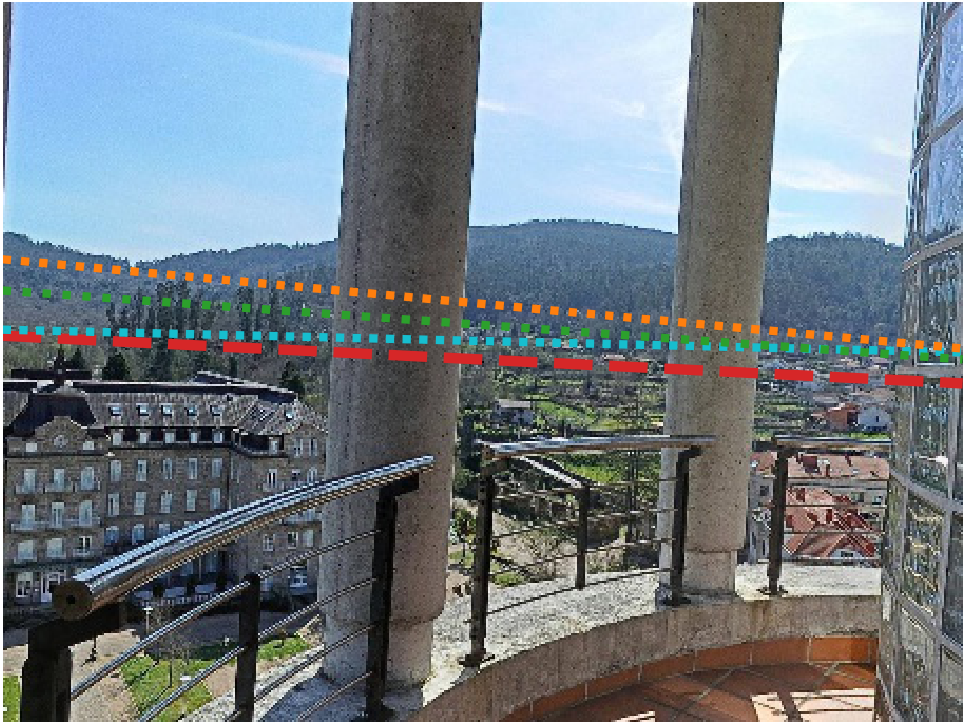
\includegraphics[width=\exampleresultswidth\linewidth]{figures/method/results/pano_addontedcyafqk_jpg-6.png} &
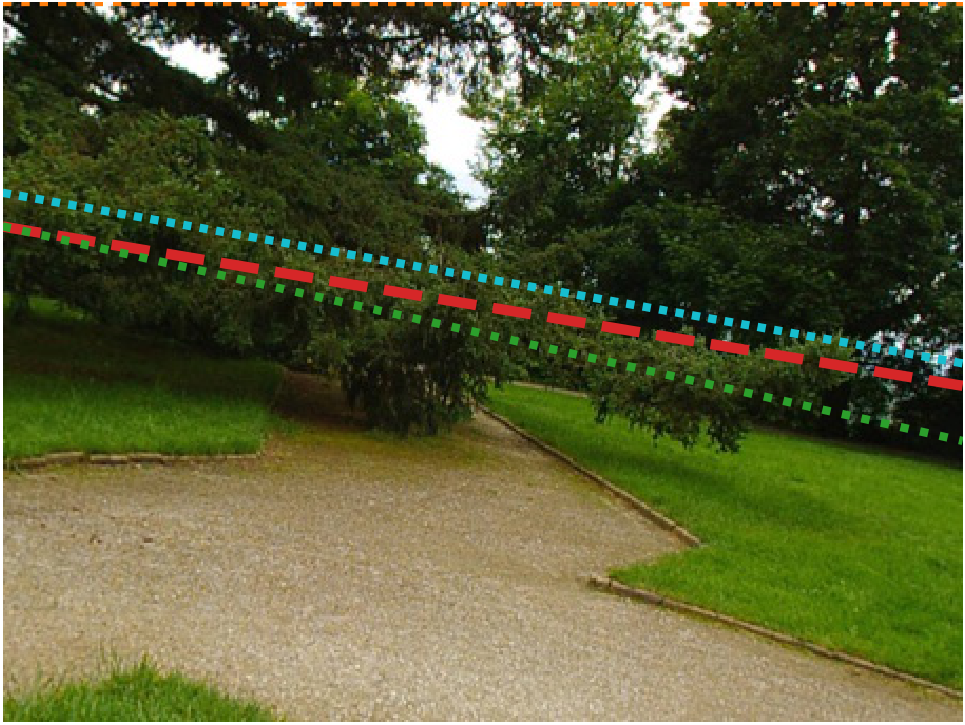
\includegraphics[width=\exampleresultswidth\linewidth]{figures/method/results/pano_addpqpwdfajota_jpg-4.png} &
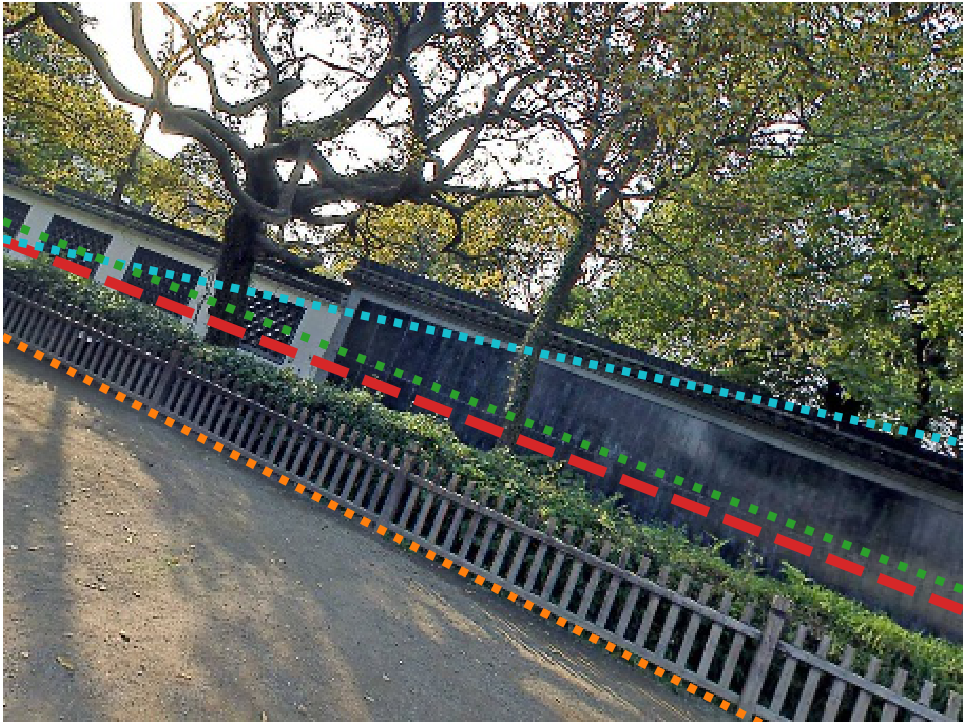
\includegraphics[width=\exampleresultswidth\linewidth]{figures/method/results/pano_addqflfuthjcbf_jpg-3.png} &
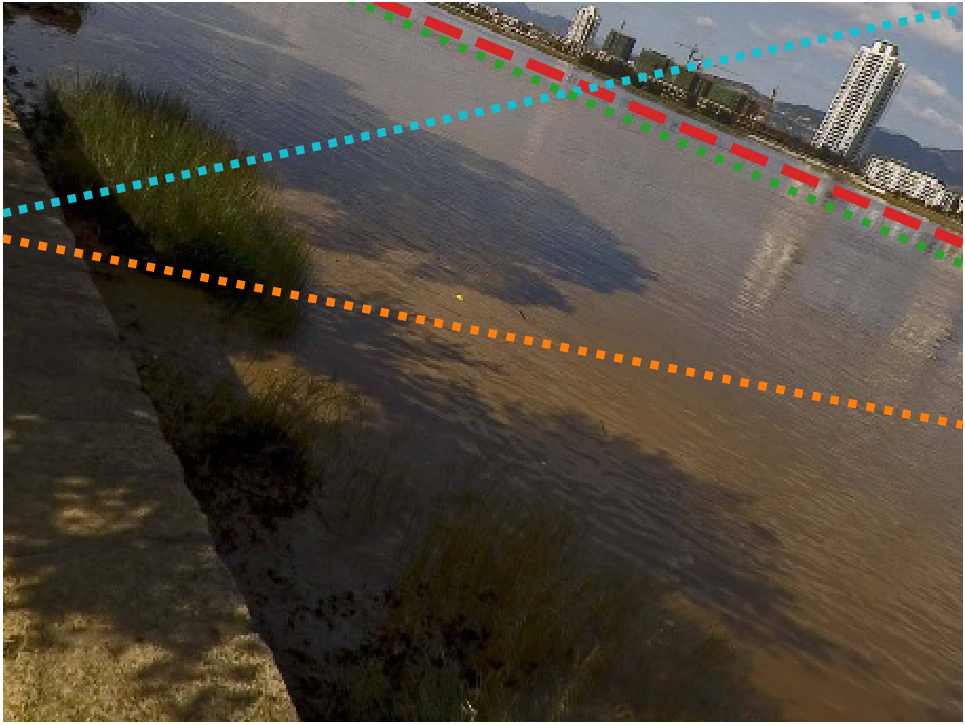
\includegraphics[width=\exampleresultswidth\linewidth]{figures/method/results/pano_adqwuqgahcnffm_jpg-0.png} &
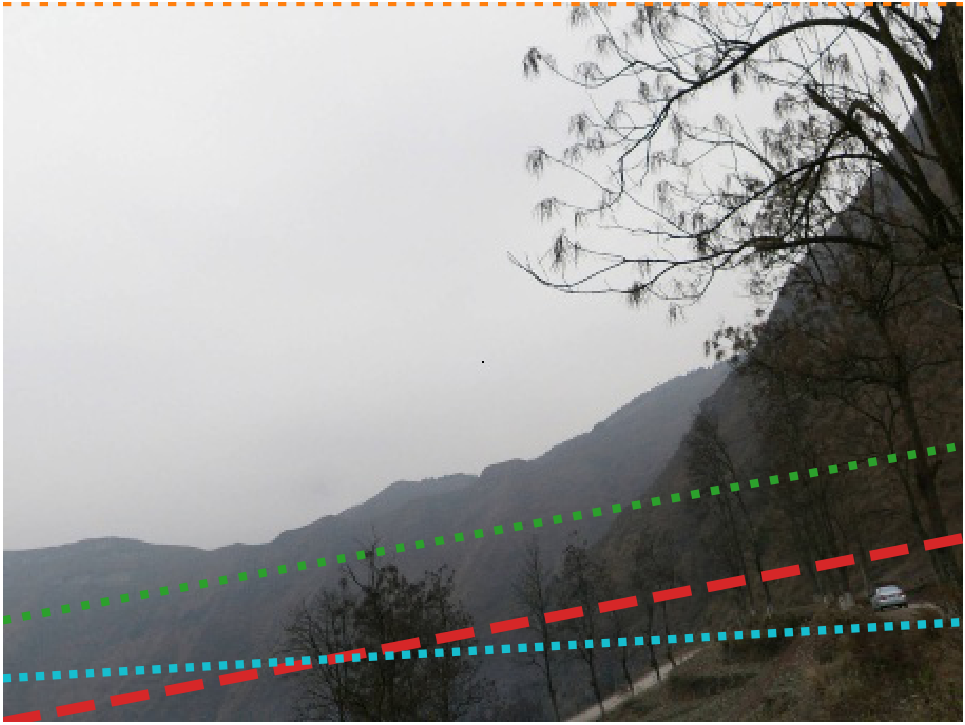
\includegraphics[width=\exampleresultswidth\linewidth]{figures/method/failures/pano_adduzncvdbrnsc_jpg-5.png} \\
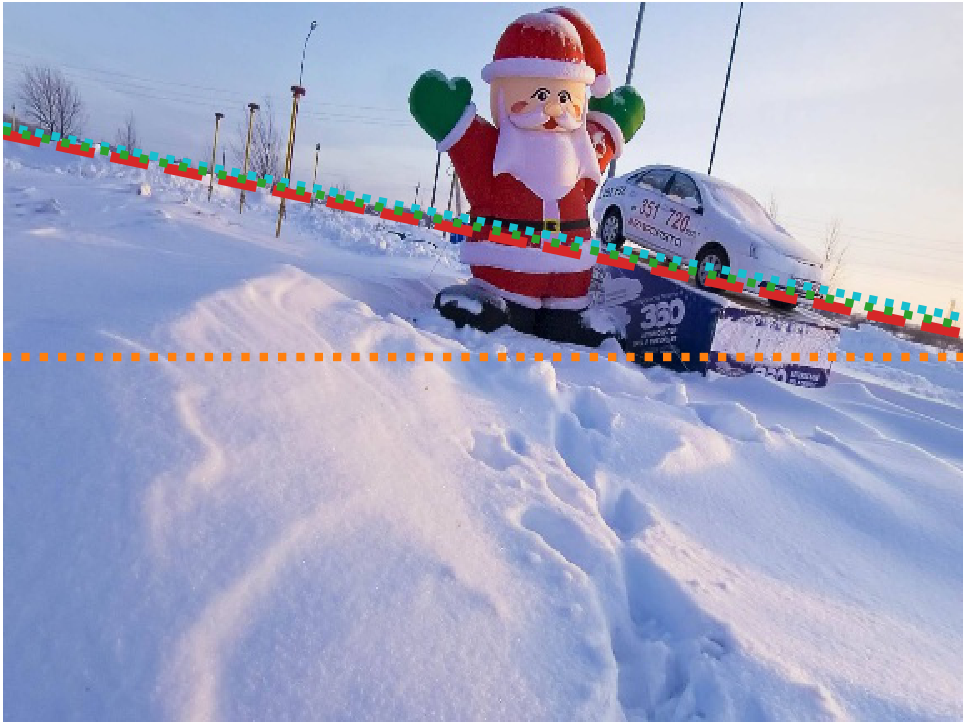
\includegraphics[width=\exampleresultswidth\linewidth]{figures/method/results/pano_addtwdtklktubg_jpg-3.png} &
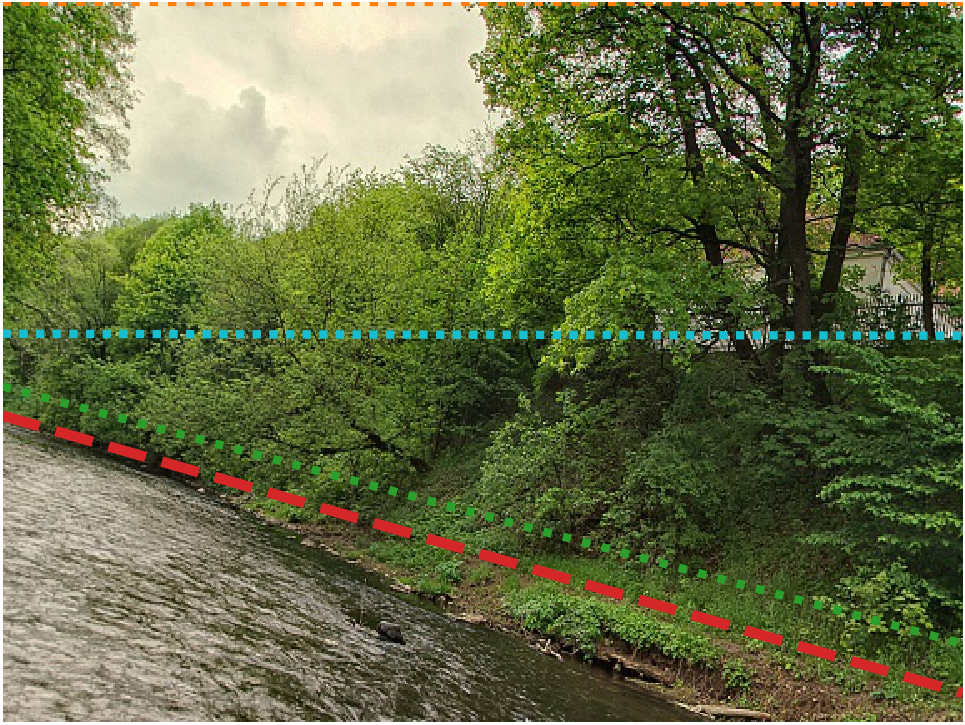
\includegraphics[width=\exampleresultswidth\linewidth]{figures/method/results/pano_addlmffiaizqlx_jpg-0.png} &
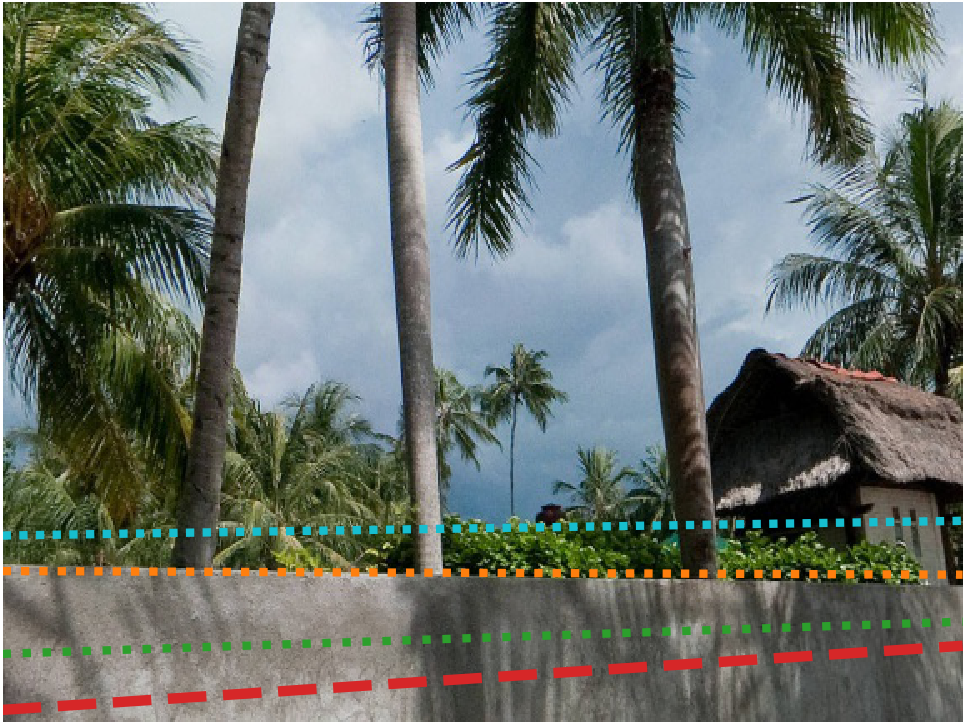
\includegraphics[width=\exampleresultswidth\linewidth]{figures/method/results/pano_addtdiecjavkue_jpg-1.png} &
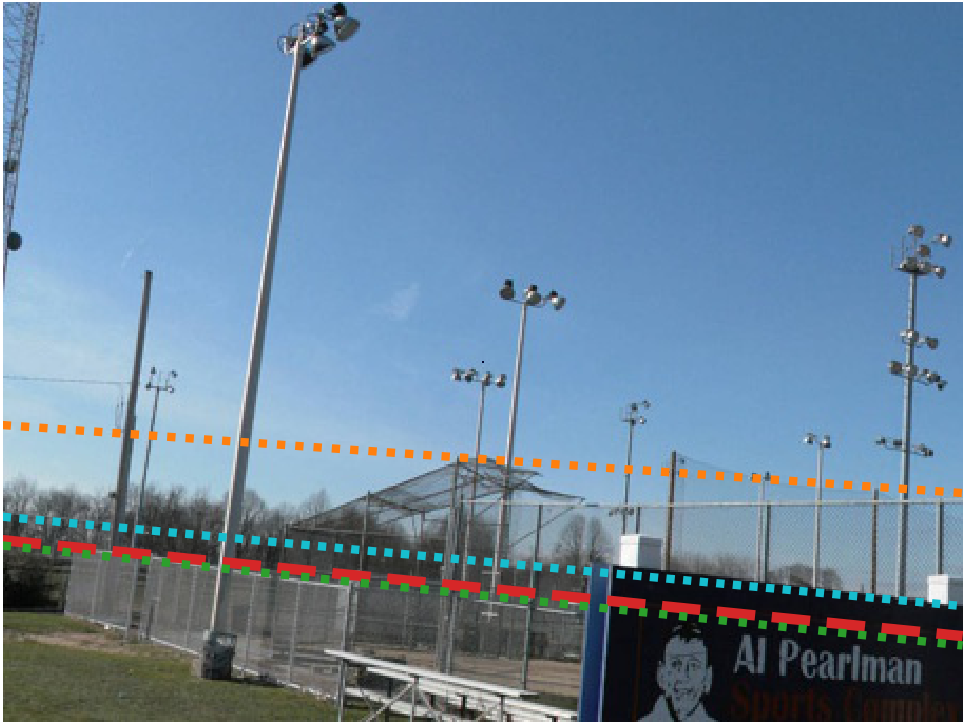
\includegraphics[width=\exampleresultswidth\linewidth]{figures/method/results/pano_ayfwzaseviqbww_jpg-2.png} &
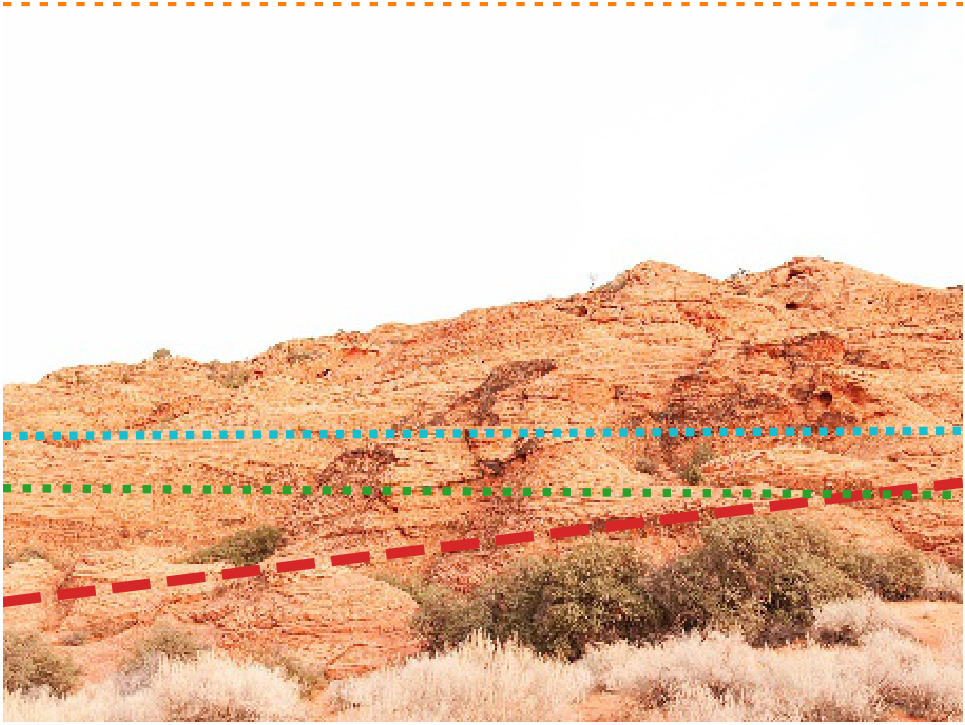
\includegraphics[width=\exampleresultswidth\linewidth]{figures/method/failures/pano_addyndxkhjhutl_jpg-3.png} \\
\multicolumn{4}{@{}c@{}}{(a)} & (b) \\
\multicolumn{5}{@{}c@{}}{
\includegraphics[trim={0 0.5cm 0.5cm 0},clip,width=0.5\linewidth]{figures/method/results/results_colorbar.pdf}}
\end{tabular}
\egroup
\caption[Example results of horizon line estimation]{Example results of horizon line estimation on the SUN360 test set. Note how Upright performs well when sharp human-made objects are present in the scene, whereas deep learned methods are more robust to organic scenes. The last column (b) contains failure cases where either the environment is not well represented in the training set (e.g. auditorium or acoustic panels) or visual cues for vanishing lines are scarce, leading to horizon estimations where humans can potentially be less sensitive to errors. \textbf{More examples available in the supplementary material.}\vspace{-1em}}
\label{fig:method_example_results}
\end{figure*}

